\chapter{Teorija} \label{chapter:teorija} 

U ovom poglavlju se obrađuje teorija Jezerskog Skladišta Podataka. Ne obrađuje
se cijela arhitektura nego samo odabrani slojevi te se daje definicija samog
Jezerskog Skladišta Podataka. Odabrani slojevi su:
\begin{itemize}
    \item Sloj Unosa Podataka,
    \item Sloj Pohrane Podataka,
    \item Sloj Obrade Podataka.
\end{itemize}
Odabirom određenih slojeva, u ovom radu se obrađuje samo dio arhitekture
Jezerskog Skladišta Podataka, ali se obrađuje teorija koja je potrebna za
razumijevanje tehnologije koja se koristi u praktičnom dijelu rada. 

\section{Jezersko Skladište Podataka} \label{section:jezersko_skladiste_podataka}

Jezersko Skladište Podataka (eng. Data Lakehouse) je arhitektura skladištenja
podataka koja kombinira karakteristike Jezera Podataka (eng. Data Lake) i
Skladišta Podataka (eng. Data Warehousea). To je centralizirano skladište
podataka koje omogućava analizu velike količine strukturiranih i
nestrukturiranih vrsta podataka u realnom vremenu ili u kasnijem trenutku.
Jezersko skladište podataka omogućuje integraciju podataka iz različitih izvora,
olakšava upravljanje podacima, smanjuje troškove i vrijeme potrebno za pripremu
podataka za analizu. Ova arhitektura skladištenja podataka postaje sve
popularnija u posljednje vrijeme jer olakšava analizu podataka, izvještavanje i
donošenje odluka u stvarnom vremenu. Za detaljniji opis Jezerskog Skladišta
Podataka vidjeti \cite{datalakehouse2022}.

\section{Sloj Unosa Podataka} \label{section:sloj_unosa_podataka}

Sloj Unosa Podataka (engl. Data Ingestion Layer) u Jezerskom Skladištu Podataka
je sloj koji se koristi za prikupljanje i spremanje podataka iz različitih
izvora u Jezersko Skladište Podataka. Ovaj sloj obuhvaća dva načina prikupljanja
podataka:
\begin{enumerate}
    \item serijsko prikupljanje podataka,
    \item strujno prikupljanje podataka.
\end{enumerate}

Sloj Unosa Podataka omogućuje podatkovnim inženjerima da učinkovito prikupe
podatke iz različitih izvora i formata, poput baza podataka, datoteka ili
senzorskih uređaja, te ih jednostavno učitaju u Jezersko Skladište Podataka.
Ovaj sloj obično uključuje alate za obradu velikih količina podataka, poput
Apache Spark-a, kako bi se omogućilo brzo i učinkovito prikupljanje i spremanje
velikih količina podataka. Za detaljni opis Sloja Unosa Podataka vidjeti
\cite{datalakehouse2022}.

\section{Sloj Pohrane Podataka} \label{section:sloj_pohrane_podataka}

U Jezerskom Skladištu Podataka, Sloj Pohrane Podataka obuhvaća skup tehnologija
i alata za pohranu velikih količina podataka u različitim formatima, kao što su
Apache Hadoop Distributed File System (HDFS), Amazon S3, Azure Blob Storage i
Google Cloud Storage.

Osim toga, Delta Lake tehnologija može se koristiti kao sloj pohrane podataka u
Jezerskom Skladištu, jer omogućuje verzioniranje podataka, upravljanje
transakcijama i omogućuje pohranu podataka u strukturiranom obliku, čime se
olakšava proces analize.

Podaci u Sloju Pohrane Podataka se dijele na 3 razine:
\begin{itemize}
    \item \textbf{Sirovi podaci/Brončani sloj} - podaci koji su prikupljeni iz izvora podataka,
    \item \textbf{Obrađeni podaci/Srebrni sloj} - podaci koji su transformirani i pripremljeni za analizu,
    \item \textbf{Analizirani podaci/Zlatni sloj} - podaci koji su analizirani i spremljeni u agregiranom obliku.
\end{itemize}

Sloj pohrane podataka u Jezerskom Skladištu Podataka mora biti dizajniran i
konfiguriran na način koji omogućuje brzi i jednostavan pristup podacima za
analizu, uz osiguravanje pouzdanosti, sigurnosti i skalabilnosti skladišta. Za
detaljni opis Sloja Pohrane Podataka vidjeti \cite{datalakehouse2022}.

\section{Sloj Obrade Podataka} \label{section:sloj_obrade_podataka} Sloj Obrade
Podataka (eng. Data Processing Layer) u Jezerskom Skladištu Podataka odnosi se
na skup tehnologija i alata koji omogućuju obradu velikih količina podataka
pohranjenih u Jezerskom Skladištu Podataka. Ovaj sloj obično uključuje
distribuirane obradne okvire, poput Apache Sparka, Apache Flinka i Apache
Beam-a.

Sloj Obrade Podataka je dizajniran kako bi omogućio izvođenje različitih
operacija na podacima, uključujući čišćenje, transformiranje, spajanje i
agregiranje. Ovaj sloj omogućuje korisnicima da lako i učinkovito izvode složenu
obradu velikih skupova podataka, koristeći alate za distribuiranu obradu.

Sloj Obrade Podataka u Jezerskom Skladištu Podataka igra ključnu ulogu u
omogućavanju pouzdane, skalabilne i brze obrade podataka pohranjenih u Jezerskom
Skladištu Podataka, što omogućuje korisnicima da izvuku vrijednost iz podataka i
donose informirane poslovne odluke. Za detaljni opis Sloja Obrade Podataka
vidjeti \cite{datalakehouse2022}.

\section{Arhitektura i tok podataka} \label{section:arhitektura_i_tok_podataka}

Arhitektura Jezerskog Skladišta Podataka prikazana je na
slici~(\ref{figure:datalakehouse_architecture}). Ona proizlazi iz slojeva opisanih
u
poglavljima~(\ref{section:sloj_unosa_podataka}),~(\ref{section:sloj_pohrane_podataka})
i~(\ref{section:sloj_obrade_podataka}). Sloj Unosa Podataka samo upisuje podatke
u Sloj Pohrane Pohrane Podataka, dok Sloj Obrade Podataka čita i piše podatke u
Sloj Pohrane Podataka. Sloj Obrade Podataka čita i piše podatke jer u tom sloju
čišćenjem, transformiranjem, spajanjem i agregiranje podataka ostvaruju
podslojevi (Brončani, Srebrni i Zlatni Sloj) Sloja Pohrane Podataka.

\begin{figure}[htb]
    \centering
    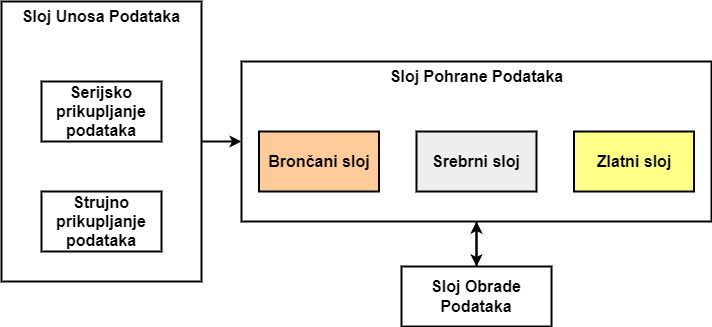
\includegraphics[width=0.8\textwidth]{images/arhitektura.drawio.png}
    \caption{Arhitektura modela Jezerskog Skladišta Podataka.}
    \label{figure:datalakehouse_architecture}
\end{figure}

Sa slike~(\ref{figure:datalakehouse_data_flow}) se vidi da postoji tok podataka
između Slojeva Unosa, Pohrane i Obrade Podataka. Sloj Unosa Podataka upisuje
podatke iz vanjske okoline (baze podataka, SFTP serveri, Jezera Podataka) u Sloj
Pohrane Podataka. Unosom podataka se dobivaju Sirovi podaci koje Sloj Obrade
Podataka dohvaća i unosi u Brončani sloj s najmanjim mogućim brojem
transformacija. Sljedeće, Sloj Obrade Podataka dohvaća podatke iz Brončanog
sloja te ih čisti, transformira i spaja. Obrađeni podaci Brončanog sloja se
unose u Srebrni sloj. Na kraju, Sloj Obrade Podataka dohvaća podatke iz Srebrnog
sloja te ih agregira i unosi u Zlatni sloj. 

\begin{figure}
    \centering
    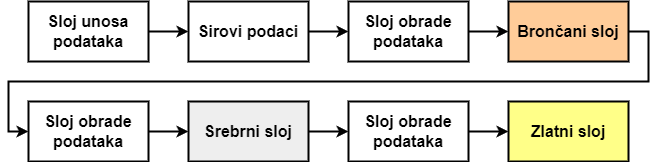
\includegraphics[width=0.8\textwidth]{images/tok_podataka.drawio.png}
    \caption{Tok podataka u Jezerskom Skladištu Podataka.}
    \label{figure:datalakehouse_data_flow}
\end{figure}